\documentclass{amsbook}
\usepackage{../HBSuerDemir}

\title{b1p1-423}
\author{Murat Buldu}
\date{October 2016}

\usepackage{mathabx}
\usepackage{graphbox}
\usepackage{mdframed}
\newmdenv[bottomline=false]{notbottom}

\begin{document}
\hPage{b1p2/423 
\footnote{Package used: mdframed for the box without bottom part}
\footnote{Package used: mathbx to get $\rightbarharpoon$ (instead we can use $\Rightarrow$ )}
\footnote{Package used: graphbox to align the images}
\footnote{Set the mdframe option:newmdenv[bottomline=false]\{notbottom\}}}

\begin{hEnumerateArabic}
    \item[]
        \begin{hEnumerateAlpha}
            \item \( { ( Ch x + Sh x )}^{- Argch x} = { ( ch x - Sh x )}^{- Argsh (x-2)}  \)
            \item \( Ch 7x + Ch 5x + Ch 3x = Ch 6x + Ch 4x + Ch 2x \)
        \end{hEnumerateAlpha}
\end{hEnumerateArabic}
\section*{ANSWERS TO EVEN NUMBERED EXERCISES}
\begin{hEnumerateArabic}
    \setcounter{enumi}{5}
    \item 24/7, 25/7, 24/25 , 7/25, 7/24, 25/24.
    \setcounter{enumi}{47}
    \item 
        \begin{hEnumerateAlpha}
            \item R, $(2x + 2) Ch(x^2 + 2)$,
            \item R, $-(2x - 2) Sech(x^2 - 2x) Th(x^2 - 2x)$
        \end{hEnumerateAlpha}
    \setcounter{enumi}{51}
    \item 
        \begin{hEnumerateAlpha}
            \begin{multicols}{2}
                \item $-\csc x$,
                \columnbreak
                \item $\csc x$
            \end{multicols}
        \end{hEnumerateAlpha}
    \setcounter{enumi}{53}
    \item
        \begin{hEnumerateAlpha}
            \begin{multicols}{2}
                \item 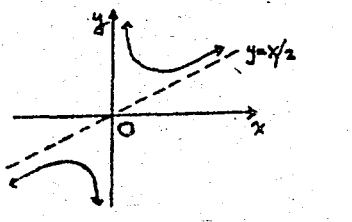
\includegraphics[align=t,scale=0.75]{images/b1p2-423-fig01.png}
                \columnbreak
                \item 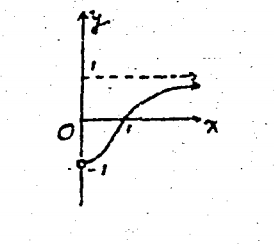
\includegraphics[align=t,scale=0.75]{images/b1p2-423-fig02.png}
            \end{multicols}
        \end{hEnumerateAlpha}
    \setcounter{enumi}{57}
    \item
        \begin{hEnumerateAlpha}
            \begin{multicols}{2}
                \item \( \ln \sqrt{3}\)  
                \columnbreak
                \item 0
            \end{multicols}
        \end{hEnumerateAlpha}
    \setcounter{enumi}{59}
    \item
        \begin{hEnumerateAlpha}
            \begin{multicols}{2}
                \item 5/4  
                \columnbreak
                \item 0
            \end{multicols}
        \end{hEnumerateAlpha}
\end{hEnumerateArabic}
\section*{A SUMMARY}
\begin{notbottom}
    \begin{hEnumerateArabic}
        \item[6.1]
            \begin{hEnumerateAlpha}{}
                \item[] \(\ln x = \int_{1}^{x} \frac{dt}{t} (x > 0), \ln 1 = 0, \ln e = 1 \)
                \item[] \(\ln ab = \ln a + \ln b, \ln \frac{a}{b} = \ln a - \ln b\)
                \item[] \(\log_b x = \log_a x \cdot \log_b a\) (change of base)
                \item[] \(\frac{d}{dx} a^{u(x)} = a^u \frac{du}{dx} \ln u, \frac{d}{dx} \log_a u(x) = \frac{1}{u} \frac{du}{dx} \log e  \)
                \item[] \(\frac{d}{dx} u(x)^{v(x)} = u^v \big(\frac{dv}{dx} \ln u +  \frac{v}{u} \frac{du}{dx} \big)  \)
                \item[] \( y = uv \ldots w \rightbarharpoon \frac{y^\prime}{y} = \frac{u^\prime}{u} + \frac{v^\prime}{v} + \ldots + \frac{w^\prime}{w} \text{(logarithmic derivative)} \)
            \end{hEnumerateAlpha}
    \end{hEnumerateArabic}
\end{notbottom}

\end{document}